\subsection{Excercise GettingStartedWithCarRentalCLI}
\label{sec:exercise_getting_started_with_car_rental_cli}
\subsubsection*{Analyze the CLI Parameters}
After analyzing the use cases presented in section 3.1 of the goLang tasks in table 4.1, the parameters displayed in figure \ref{fig:car_rental_cli_parameters} are needed.

\begin{figure}[H]
    \centering
    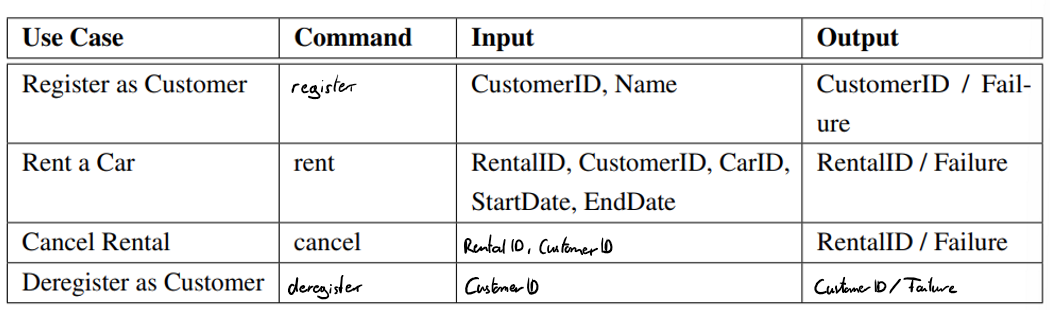
\includegraphics[width=\textwidth]{figures/goLang/carRental/carRental_CLIParameters.png}
    \caption{CLI Parameters}
    \label{fig:car_rental_cli_parameters}
\end{figure}

\subsubsection*{Describe the Software Architecture}
The given task starts with three different software components:
\begin{itemize}
    \item Presentation Layer: CarRentalCLI
    \item Application Logic Layer: CarRentalOperations
    \item Infrastructure Layer: CarRentalRepository
\end{itemize}
\subsubsection*{Presentation Layer: CarRentalCLI}
\begin{itemize}
    \item Functionality: This component implements the CLI itself. 
          It creates a new CLI object, runs it, and exits safely if an error occurs.
          Furthermore, it implements the CLI commands with the list of according functions a command calls.
    \item Interfaces: The CLI component implements the CarRentalOperationsInterface
    \item Dependencies: This layer is dependent from the applications logic layer, importing and implementing functions from the logic layer.
    \item Reusability: The layer is reusable since it only implements CLI and commands.
          By providing a different set of function the CLI implements, one can reuse the CLI in a different context.
    \item Scalability and Maintainability: It can be scaled by adding new commands and functions to the CLI.
          It can be maintained by fixing commands and the according functions.
          By separating the CLI into a single layer, the commands can be organized systematically and provide great overview.
\end{itemize}

\subsubsection*{Application Logic Layer: CarRentalOperations}
\begin{itemize}
    \item Functionality: This component implements the business logic of the application.
          It provides functions for the CLI to call, which then call the according functions from the infrastructure layer.
          It also provides the models of the objects, that are used in the application.
    \item Interfaces: This component implements the CarRentalRepositoryInterface and provides the CarRentalOperationsInterface
    \item Dependencies: This component is dependent from the infrastructure layer and therefore dependent from the layer below.
    \item Reusability: Since this component uses the infrastructure layer, it is not directly reusable.
          It implements a specific set of functions, which cannot be reused in different contexts.
    \item Scalability and Maintainability: It can be scaled by adding new functions to the component.
          It can be maintained by fixing functions.
\end{itemize}

\subsubsection*{Infrastructure Layer: CarRentalRepository}
\begin{itemize}
    \item Functionality: This component implements yaml mappers and entities. 
          This allows for simple communication between the application and the yaml files.
          The yaml mappers provide functions to read and write yaml files.
          The entities provide the structure of the yaml files and the structure of the struct the mapper creates.
    \item Interfaces: This component provides the CarRentalRepositoryInterface
    \item Dependencies: The component is dependent from the provided yaml files, since it reads and writes them.
          In terms of functionality, no functionality imports from other parts of the application are needed since all functions are implemented in the component itself.
    \item Reusability: This component is reusable since it only implements yaml mappers and entities.
          By providing a different set of entities and mappers, one can reuse the component in a different context.
    \item Scalability and Maintainability: By adding new mappers and entities, the functionality can be extended.
          By fixing the mappers and entities, the maintainability can be ensured.
\end{itemize}

\subsubsection*{Analyze the Micro Architecture}

\subsubsection*{Start the Go Program CarRentalCLI}
The output after starting the program successfully is displayed in figure \ref*{fig:car_rental_cli_successful_rental_max}.
The program asks for the id of the customer and the id of the car.
After entering the ids, the program asks for the start and enddate of the rental by asking for the day, month and year.
If the data is entered correctly and the rental is successful, the program prints a success message and exits.
Otherwise, the program asks for the remaining data, prints an error message, the exit-status and exits.

\begin{figure}
      \centering
      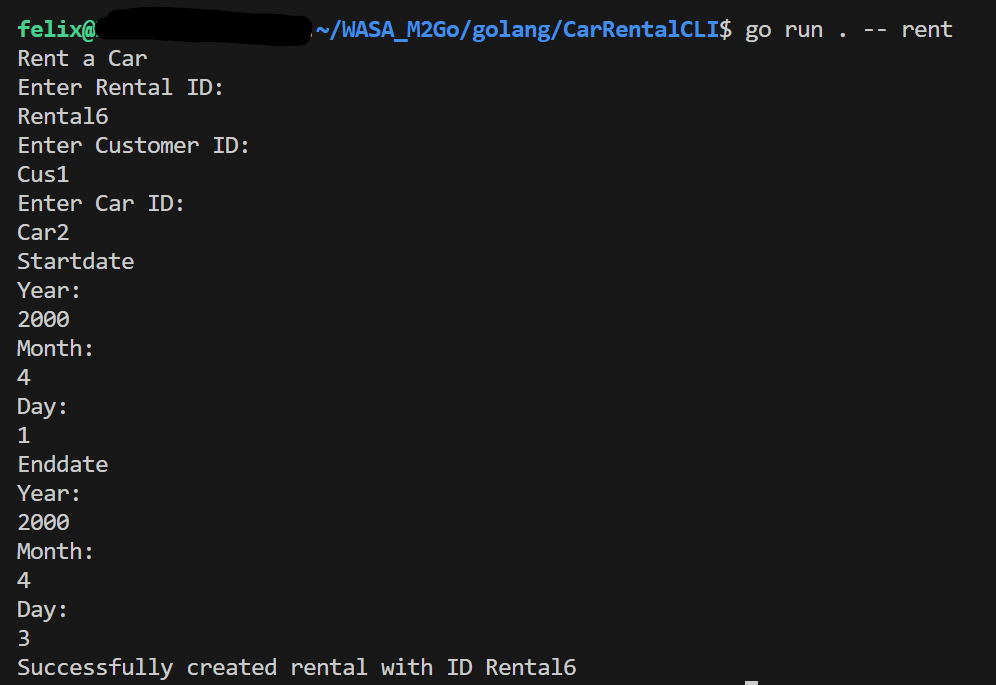
\includegraphics[width=0.8\textwidth]{figures/goLang/carRental/carRentalCLI/carRentalCli_SuccessfulRentalMax.png}
      \caption{Successful Rental of a Car for Max}
      \label{fig:car_rental_cli_successful_rental_max}
\end{figure}

\subsection{Excercise AddRegisterAsCustomer}
\label{sec:exercise_add_register_as_customer}
\subsubsection*{Why is the Mapper required?}
The general task of a mapper is to enable communication between the application and the database.
In this case, the database is a yaml file.
Therefore the mapper can read and write to the yaml files and convert the data to the according entities and vice versa.

In the use case of registering a new customer, the mapper is called while creating a new customer.
The yaml mapper receives the customer object from the function and returns the CustomerPersistenceEntity.
This entity is then written to the yaml file.
By writing the entity into the yaml file, the customer is registered and can be used in the application.

\subsubsection*{Register Alice as Customer}
After running the CLI command to register a new customer, the program asks for the ID of the customer.
In this case Alice receives the ID \texttt{Cus5}.
After entering the ID, the program asks for the name of the customer, in this case Alice.
The program exits with a success message and the exit-status as shown in figure \ref{fig:car_rental_cli_register_alice}.

To register a new rental, the programm starts with \texttt{go run . -- rent}.
The program asks for the ID of the rental, here it is \texttt{Rental7}.
The customer ID for Alice is \texttt{Cus5}.
After that the start and enddate is entered.
The program exits with a success message and the exit-status as shown in figure \ref{fig:car_rental_cli_rental_alice_successful}.

\begin{figure}
      \centering
      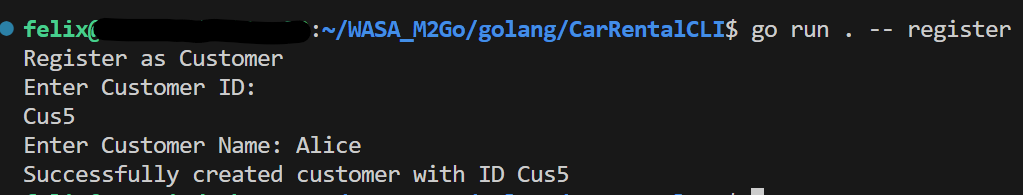
\includegraphics[width=0.8\textwidth]{figures/goLang/carRental/carRentalCLI/carRentalCLI_RegisterAlice.png}
      \caption{Register Alice as a Customer}
      \label{fig:car_rental_cli_register_alice}
\end{figure}
\begin{figure}
      \centering
      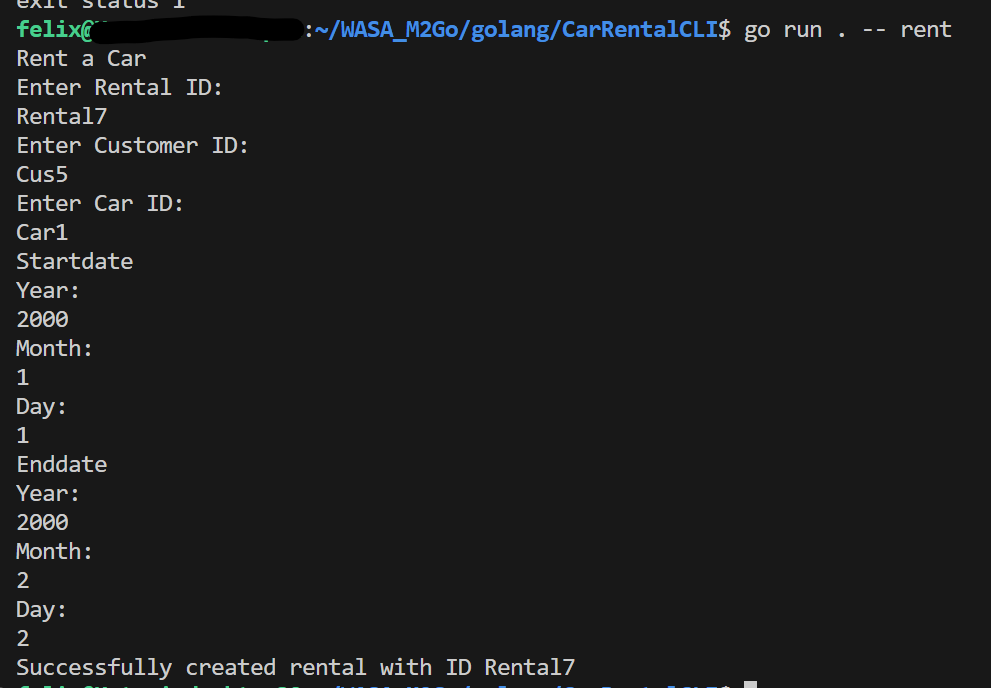
\includegraphics[width=0.8\textwidth]{figures/goLang/carRental/carRentalCLI/carRentalCLI_SuccessfulRentalAlice.png}
      \caption{Successful Rental of a Car for Alice}
      \label{fig:car_rental_cli_rental_alice_successful}
\end{figure}
